\begin{figure}
  \centering
  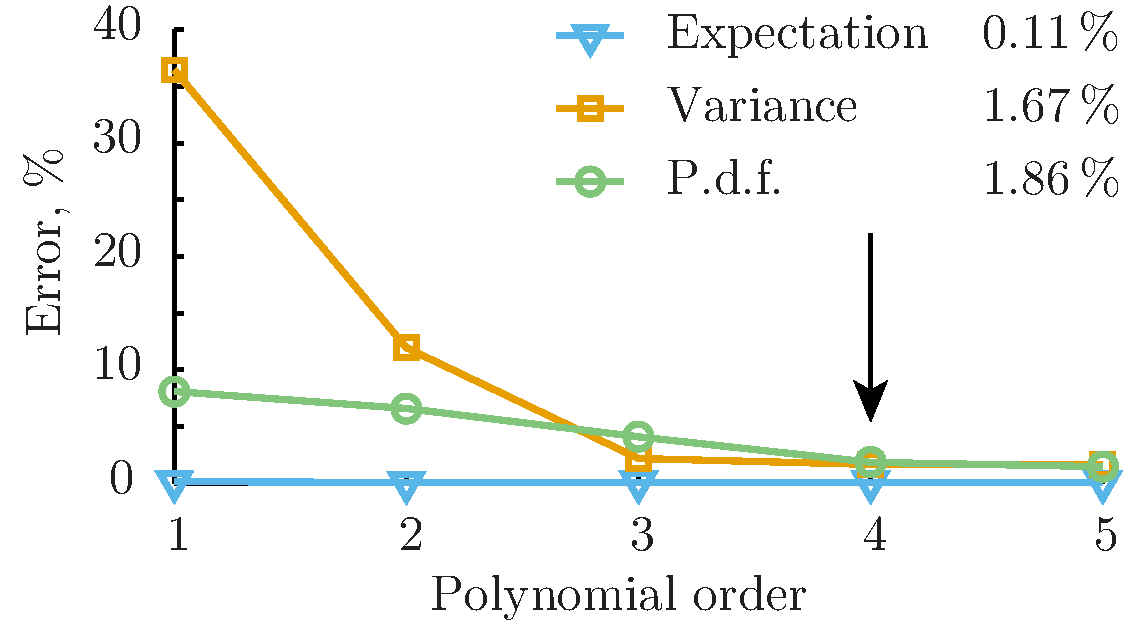
\includegraphics[width=1.0\columnwidth]{include/assets/accuracy.pdf}
  \caption{Errors of expectation, variance, and \pdf}
  \flabel{accuracy}
  \vspace{-1.6em}
\end{figure}

The construction of PC is based on the Hermite polynomial basis (see \tref{askey}) as it was found to be optimal in many situations involving Gaussian parameters \cite{xiu2002}. A one-dimensional example of the basis is given in \fref{hermite} where the first six Hermite polynomials $\{ \pcb_i(\z) \}_{i = 1}^6$ are displayed.

Once the basis has been chosen, we need to compute the corresponding coefficients, specifically, $\pcc{\vP}_i$ in \eref{pc-expansion}. As shown in \aref{polynomial-chaos}, $\pcc{\vP}_i$ involve multidimensional integration with respect to the \pdf\ of the \rvs\ $\vZ(\o)$. In numerical analysis, this task is typically accomplished by virtue of a quadrature rule \cite{press2007}, which, loosely speaking, is a weighted summation over the integrand values computed at prescribed points. A natural choice of a quadrature rule when the weight function is a Gaussian \pdf\ is the Gauss-Hermite quadrature. For clarity of presentation, a detailed explanation of the computational procedure is left to the appendix, \aref{gauss-quadrature}, in which an introduction to numerical integration and, in particular, to Gauss quadratures is given.

To summarize, we have completed four out of five steps of the proposed UQ framework depicted in \fref{algorithm}. The result is a light surrogate of the problem in \eref{fourier-system}. More precisely, at each moment of time, the surrogate is composed of two $\cores$-valued polynomials, one for power and one for temperature, that are defined in terms of $\vars$ mutually independent \rvs; an example of such a polynomial is given in \eref{pc-k}. The constructed representation can now be trivially analyzed to retrieve various statistics of the stochastic system in \eref{fourier-system}, and this is the fifth step in \fref{algorithm}, which we shall discuss in the following section.
